\section{Second data set}

This section of the report uses data from the study \citetitle{Cohen:2010} by \citeauthor{Cohen:2010}
\citeyear{Cohen:2010} \cite{Cohen:2010}.  The analysis here looks to a deeper understanding of the
data by using centile estimation.  This will allow the exploration of how relationships between
variables manifest across different segments of the data distribution, rather than just focusing on
mean effects.

\subsection{Distribution Overview}

\subsubsection{Box-Cox Cole and Green: \texttt{BCCG}}
The starting  distribution for this analysis is the \textbf{Box-Cox Cole and Green} (\textbf{\texttt{BCCG}}) distribution.  This satisfies
the requirements when using the LMS method of centile estimation of Cole and Green \cite{Rigby:2019}.  It does this by using a transformation
to a normal distribution \citeauthor{Box:1964} \cite{Box:1964}.

\subsubsection{Box-Cox \emph{t}: \texttt{BCT}}

To add kurtosis modeling to the LMS method, we can use the \textbf{Box-Cox \emph{t}} (\textbf{\texttt{BCT}}) distribution.  This transforms the
random variable $Z$ so it follows a truncated distribution, with degrees of freedom $\tau$ treated as a continuous parameters.
This gives a good model for response variables $Y$ on $(0, \infty)$ when $Y$ is not very close to zero \cite{Rigby:2019}.

\subsubsection{Box-Cox Power Exponential: \texttt{BCPE}}

Also adding kurtosis is the \textbf{Box-Cox power exponential} (\textbf{\texttt{BCPE}}) distribution.  This uses a
transformed random variable $Z$, following a truncated standard power exponential distribution, with the power parameters $\tau > 0$
treated as a continuous parameter.  This gives a flexible distribution for a response variable $Y$ on $(0, \infty)$ also when $Y$ is not very
close to $0$ \cite{Rigby:2019}. 

\subsection{Fitting the Distributions}

The BCCG distribution is chosen for its flexibility in modeling skewed data, which is often encountered in physical measurements
like grip strength. By adjusting for age with P-splines, the model can flexibly accommodate nonlinear age effects on the
distribution parameters of grip strength, making it a powerful approach for analyzing such data.


\subsubsection{Transformations of Grip against Age}

We don't see an need for transformations on the grip vs age relationship.   When fitting models, it is a good guide to keep models a
s parsimonious and simple as possible, whist fitting the data well.

The general guidelines for not needing a power transformation are:
\begin{itemize}
\item  Linearity: If the relationship between age and grip strength is linear or close to linear, applying a
  transformation to age would not yield any significant benefits in terms of linear regression modeling or interpretation.
\item  Variability: Power transformations are also used to stabilize variance across the range of predictor variables.
  If the variance of grip strength is relatively constant across ages, then transforming age wouldn't help in stabilizing variance.
\item  Normality of Residuals: Another reason for transformations could be to achieve normality of residuals in regression
  modeling. If the residuals from a model with age predicting grip strength are already approximately normally distributed,
  a transformation is unnecessary.
\item  Simplicity: Avoiding unnecessary transformations keeps the model simpler and makes interpretation more straightforward.
  If a simple model without transformation provides satisfactory results, it's often preferred for ease of
  explanation and understanding.
\end{itemize}

\begin{figure}[H]
  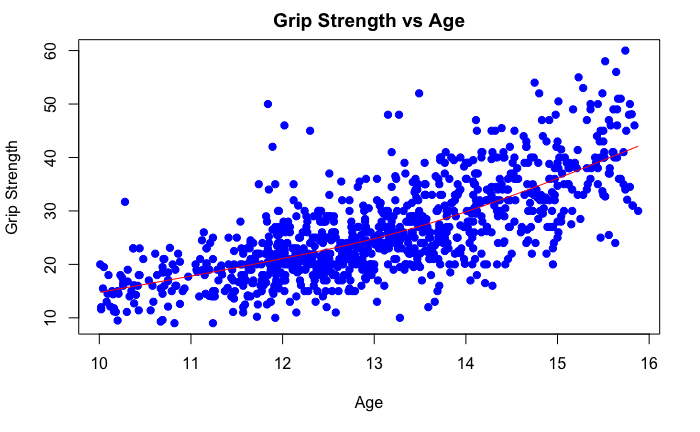
\includegraphics{q2_grip_vs_age.png}
  \caption{Plot of Grip Strength vs Age}
\end{figure}

Looking at a plot of the grip we can see a generally linear relationship with age. There looks to be a change in variance
across age, but not large enough to mandate a power transformation.

\subsubsection{Interpreting the Effective Degrees of Freedom}

\begin{table}[H]
\begin{verbatim}
                    BCCG EDF    BCT EDF     BCPE EDF

$mu$`pb(age)`       4.574796    4.627933    4.73276

$sigma$`pb(age)`    2.002746    2.002241    2.002326

$nu$`pb(age)`       2.000129    2.000142    2.000113

$tau$`pb(age)`                  2.839583    2.948827

\end{verbatim}
\caption {Effective degrees of freedom for models}
\end{table}

An EDF near 1 suggests that the model is applying very little smoothing to that parameter and can imply a linear relationship
between the parameter and the predictors.

When significantly greater than 1, the EDF indicates more complex relationships are being modeled, with the splines applying
more smoothing. This is often necessary when the relationship between the response and predictors is nonlinear or when there's
a varying effect of predictors across the range of the data.

Very high EDF values, though, may signal overfitting, where the model is too closely fitting the idiosyncrasies of the sample
data rather than capturing the underlying population trends.

What we seem to see here is that mu ($\mu$/location), sigma ($\sigma$/scale or dispersion), nu ($\nu$) and tau ($\tau$) (controlling
the shape of the distribution, including skewness and kurtosis) are all indicating that the relationships are being modeled
without over-fitting the data.


\subsection{Selection of Distribution}

Across the three scoring metrics of GAIC, centile plots, and residuals analysis, the BCPE model best captures the dynamics of the
data.  Both kurtosis models perform better than the baseline BCCG model, but the BCPE captures that data dynamics better than the
BCT model.

\subsubsection{Investigate Fitted Model Residuals}


\begin{figure}[H]
  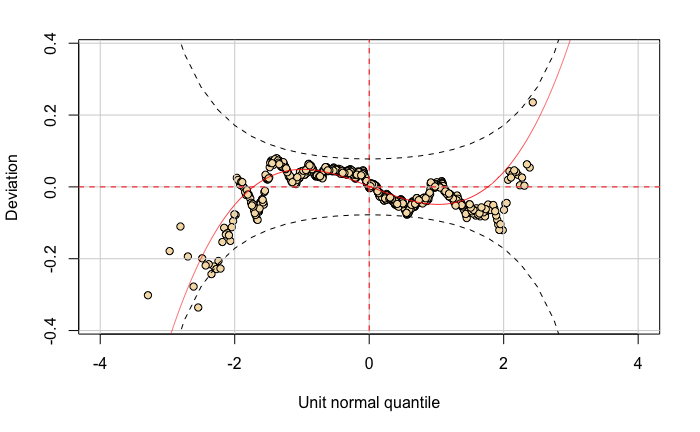
\includegraphics{q2_bccg_wp.png}
  \caption{Residuals worm plot for the BCCG model}
\end{figure}


\begin{figure}[H]
  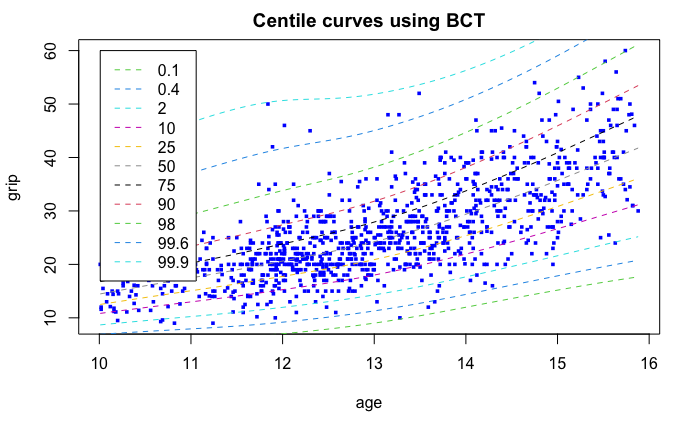
\includegraphics{q2_bct_wp.png}
  \caption{Residuals worm plot for the BCT model}
\end{figure}


\begin{figure}[H]
  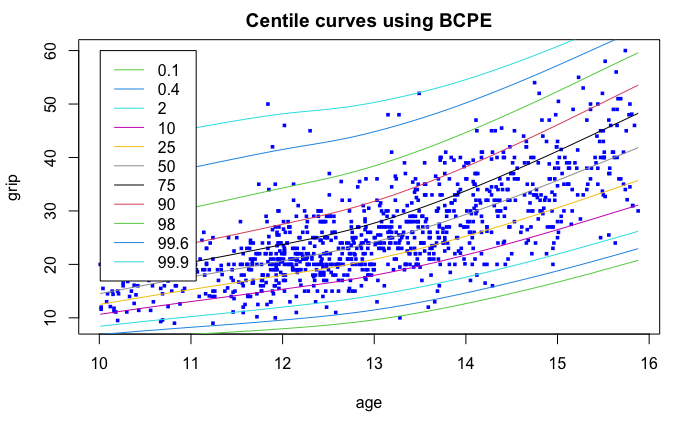
\includegraphics{q2_bcpe_wp.png}
  \caption{Residuals worm plot for the BCPE model}
\end{figure}

These worm plots should ideally resemble a straight line. Any curvature or deviations from the line indicates potential
issues with the model's fit to the data, such as non-normality or heteroscedasticity.

We would like to see randomly distributed residuals, around zero, and without clear patterns.  BCCG is obviously the worst
performing model, with far more pronounced curvature.  The BCT model performs better, but the BCPE has the straightest plot
and slightly less extreme residuals on the outlining points.


\subsubsection{GAIC Scoring}

The GAIC is a variant of the Akaike Information Criterion (AIC) that allows for a more flexible penalization of
model complexity and is particularly useful in comparing models fitted with the same dataset but
different distributions or complexities.

\begin{table}[!ht]
\begin{verbatim}
[1] "GAIC for BCCG: 6332.69897370389"
[1] "GAIC for BCT:  6321.12544775062"
[1] "GAIC for BCPE: 6317.44993530573"
\end{verbatim}
\caption {GAIC results for BCCG, BCT \& BCPE models}
\end{table}

We find that the BCPE model has the lowest GAIC, indicating that it strikes the most favorable balance between model
fit and complexity. The GAIC penalizes models more heavily
for additional parameters than the traditional AIC does, making it particularly useful for models that might overfit
the data with too many parameters or excessive flexibility.

\subsubsection{Centile Plots for Fitted Models}

\begin{figure}[H]
  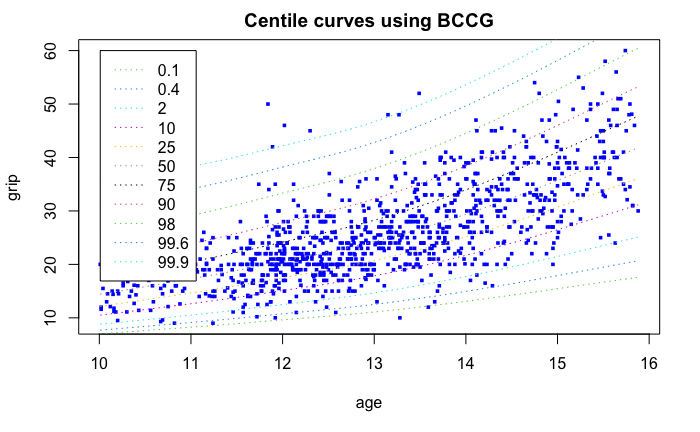
\includegraphics{q2_bccg_centiles.png}
  \caption{Centile curves for BCCG model}
\end{figure}


\begin{figure}[H]
  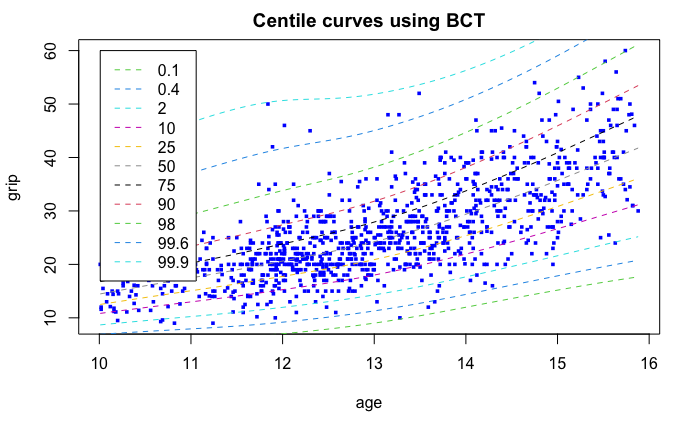
\includegraphics{q2_bct_centiles.png}
  \caption{Centile curves for BCT model}
\end{figure}



\begin{figure}[H]
  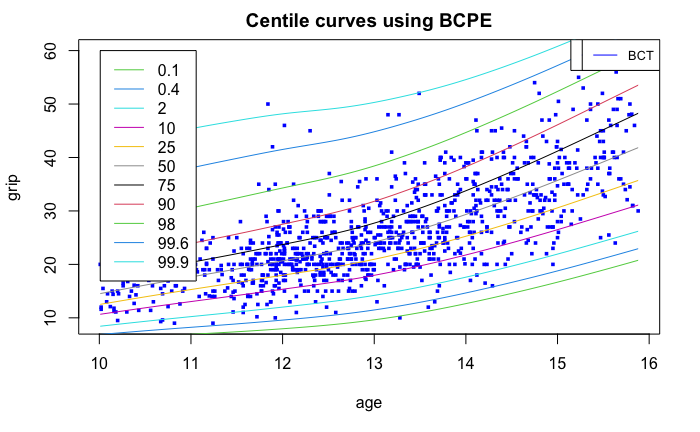
\includegraphics{q2_bcpe_centiles.png}
  \caption{Centile curves for BCPE model}
\end{figure}

Looking at the centile plots, we get a visual representation of how each model performs across the age spectrum.

The most obvious artifact of these plots is that there's a broad overlap for the upper age groups, above 14 years.  Visually
we can see less outliers in these older ages, whilst in the younger ages we see outliers.

The BCT model manages to capture all observations in the $(0.1, 99.1)$ centile bands, whilst the BCPE model is slightly
tighter, allowing some extreme outliers to remain outside that band.  Our baseline BCCG, which does not admit kurtosis, is
narrower again, indicating that the model is failing to explain these observations.  As kurtosis in a distribution allows
more extreme values than a normal distribution, this makes sense that the BCCG model does more poorly in the GAIC scoring.
